
Continuing our quest for a fast kNN search, a parallelization of the k-d tree build was introduced with RQ~\ref{rq:parallel_build}, in Section~\ref{sec:development_of_a_parallel_k_d_tree_build_algorithm}.

\textbf{RQ~\ref{rq:parallel_build}.} \emph{It is possible to parallelize the k-d tree build algorithm, in such a way that it gives a significant speed improvement compared to the serial algorithm.}

The resource question is based around the complex nature of the k-d tree build, and the uncertainty of a acceptable parallel speedup. This question was investigated though implementation prototypes, together with a thorough discussion about the parallelization and the intermediate results. 



\begin{figure}[ht!]
    \centering
    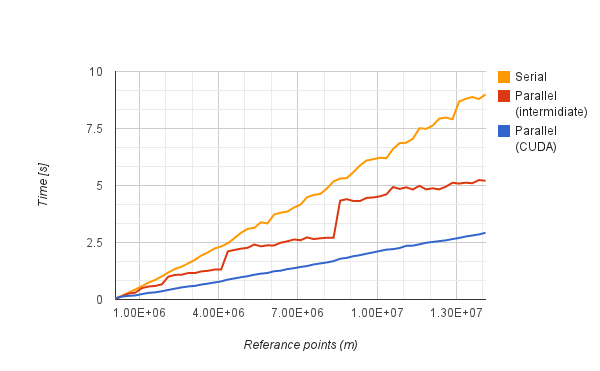
\includegraphics[width=120mm]{../gfx/final_tree_build.png}
    \caption{Comparison between serial and parallel k-d tree build performance.}
    \label{fig:final_tree_build}
\end{figure}

Figure~\ref{fig:final_tree_build} tries to answer RQ~\ref{rq:parallel_build}, by comparing the serial and parallel k-d tree build implementation. Both graphs follows the same trend, which correlates with the shared time complexity of \BigO{m\ log(m)}. We see that the impact of the parallel overhead is decreasing as the problem size increase, as the profit of multiple cores is getting more and more be dominant. Resulting in a faster parallel implementation.

To get a better picture of the parallel improvement, it is natural to talk about parallel speedup. Figure~\ref{fig:final_tree_build_speedup} shows how the parallel speedup develops, as the problem size increase. The speedup starts below $1$, indicating that the serial version is faster, but from Figure~\ref{fig:final_tree_build} one can see that the time to build such small k-d trees is almost negligible. As the problem size increase, the trend quickly changes, until the speedup flattens out. This is a typical scenario in this kind of speedup graphs. The speedup increases as the problem size allows utilization of more and more threads, until the limit is reached, and the curve flattens out into a lower gradient. Our implementation reach this flattening at a parallel speedup of around $3$.      

\begin{figure}[ht!]
    \centering
    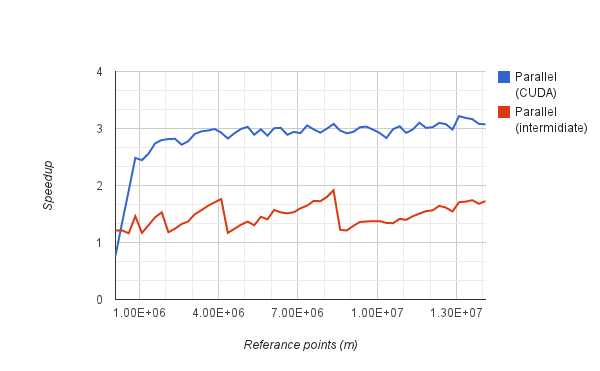
\includegraphics[width=120mm]{../gfx/final_tree_build_speedup.png}
    \caption{Parallel speedup for the k-d tree implementation for varying values of $m$.}
    \label{fig:final_tree_build_speedup}
\end{figure}

With the complex nature if a k-d tree build process, a speedup of $3$ is acceptable, and we categorize it as a significant improvement. We can therefore conclude that the answer to RQ~\ref{rq:parallel_build} is yes. 


\textbf{RQ~\ref{rq:parallel_query}.} \emph{It is possible to parallelize the All-kNN query algorithm, in such a way that it gives a significant speed improvement compared to the serial algorithm.}


\begin{figure}[ht]
    \centering
    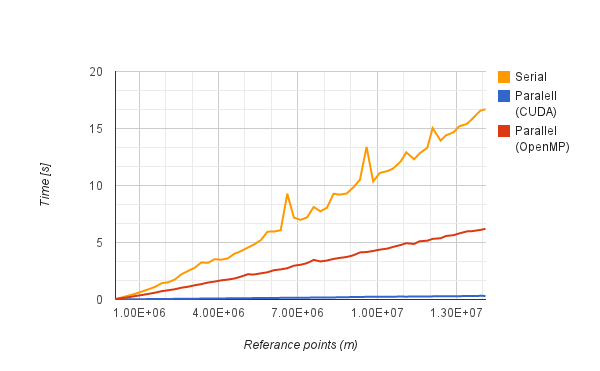
\includegraphics[width=120mm]{../gfx/final_kd_search.png}
    \caption{Comparison between serial and parallel All-kNN query performance.}
    \label{fig:final_kd_search}
\end{figure}

\begin{figure}[ht]
    \centering
    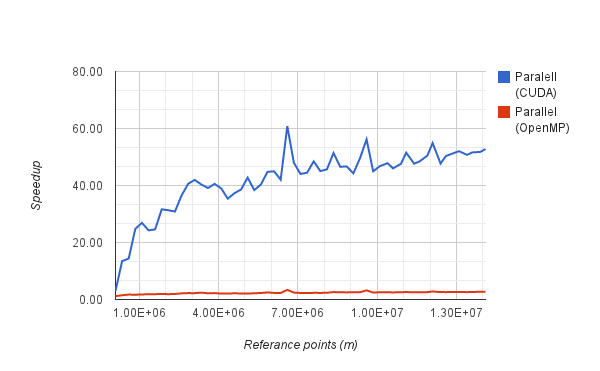
\includegraphics[width=120mm]{../gfx/final_kd_search_speedup.png}
    \caption{Parallel speedup comparison for the All-kNN query between the CUDA and OpenMP implementation.}
    \label{fig:final_kd_search_speedup}
\end{figure}



Graph of serial and parallel build, and query.

Some speedup calculation. Include Garcia as well, and point out that high speedup does not equal fast algorithm.
